% Appendix of main.tex: tests and convergence of the moment transport.
% Condensed from convergence.tex (Sections 2-3). Figure: scripts/fig_app_convergence.py.
\section{Tests and convergence of the moment transport}\label{app:convergence}

\begin{figure}[h]
\centering
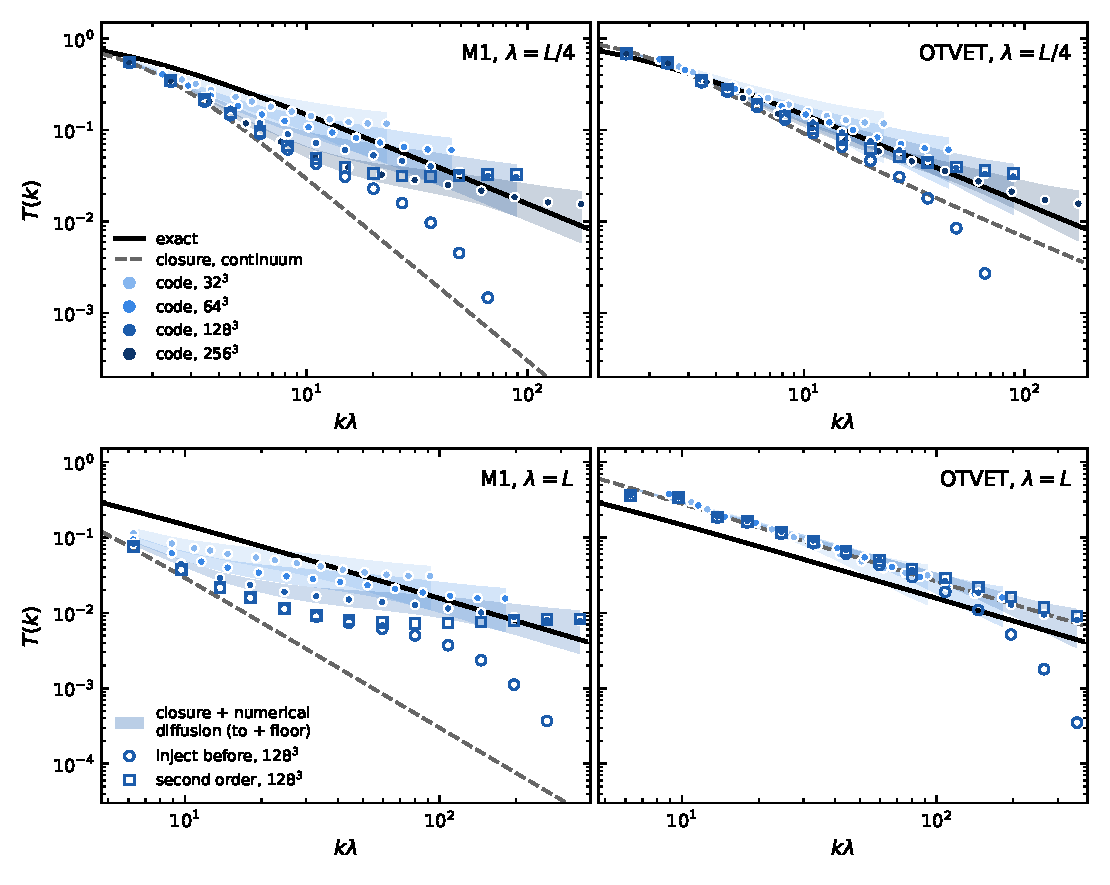
\includegraphics[width=0.9\linewidth]{figures/fig_app_convergence.pdf}
\caption{Transfer function from the sources to the photon density for a uniform mean free path $\lambda$,
with a source in every cell: M1 (left) and OTVET (right), $\lambda=L/4$ (top) and $\lambda=L$ (bottom), where $L$ is the boxsize.
Black: the exact solution, equation~(\ref{eq:app_exact}). Dashed: the linear solution of each closure in
the continuum, equations~(\ref{eq:app_m1}) and (\ref{eq:app_otvet}). Filled blue circles: our moment
transport with the settings of the suite and a source in every cell, at $32^3$ to $256^3$ cells (light to
dark). Thin blue curves: the linear solution of the discretized equations at
each resolution, equation~(\ref{eq:app_disc}). Open blue symbols, $128^3$ only: sources injected before the
transport (circles; dotted curve: its linear solution) and a second-order scheme (squares). Right: the ray
tracer at $128^3$ with sources in one cell in 512, for pools of 8, 15 (the suite), 64 (the original) and
120 rays per cell (light to dark). Thin curves: the exact solution plus white noise of rms
$0.95\,n_{\rm ray}^{-1/2}$ per cell. Open circles: the pool of 15 averaged over 16 substeps.}
\label{fig:app_conv}
\end{figure}

We test the transport as \citet{gnedin25} does, with a uniform mean free path
$\lambda=1/\kappa$ in a periodic box of side $L$. The moment transport routines of the code are run to steady
state with a source of random luminosity in every cell (30\% rms), and each substep (one cell of light
travel, $\Delta t=\Delta x/\chat$, taken in four transport updates) ends with $N$ and $\mathbf F$ multiplied
by $e^{-\Delta x/\lambda}$ in place of the chemistry. We measure
$T(k)\equiv[P_N(k)/P_L(k)]^{1/2}$, normalized to unity as $k\to0$; with uniform opacity this is the
$T_{\Gamma L}$ of Section~\ref{sec:conclusions}. Figure~\ref{fig:app_conv} compares it with the following
analytic results.

\emph{Exact.} Each source contributes $L_se^{-r/\lambda}/(4\pi r^2\chat)$ to $N$, whose Fourier
transform gives
\begin{equation}
T_{\rm exact}(k)=\frac{1}{\lambda}\int_0^\infty\!dr\,e^{-r/\lambda}\,\frac{\sin kr}{kr}
=\frac{\arctan(k\lambda)}{k\lambda}.\label{eq:app_exact}
\end{equation}

\emph{The closures in the continuum.} In steady state the moment equations are
$i\mathbf k\cdot\mathbf F=S/\chat-\kappa N$ and $ik_j(\mathsf D_{ij}N)=-\kappa F_i$. With many sources
per $\lambda^3$ the radiation is nearly isotropic, and M1 has $\mathsf D=\mathsf I/3$ to first order in
the perturbation, so
\begin{equation}
T_{\rm M1}(k)=\frac{1}{1+k^2\lambda^2/3},\label{eq:app_m1}
\end{equation}
which falls as $3/(k\lambda)^2$ where the exact solution falls as $\pi/(2k\lambda)$. The OTVET tensor
(equation~\ref{eqn:otvet}) instead responds to the sources: for source fluctuations $\delta_L$,
$\delta\mathsf D_{ij}(\mathbf k)=-(\pi^2/kL_{\rm O})(\hat k_i\hat k_j-\delta_{ij}/3)\,\delta_L(\mathbf k)$
for $kL\gg1$, where $L_{\rm O}\equiv\int d^3r/r^2=7.66\,L$ over the minimum-image cube. This adds a term to
the flux equation and gives \citep{wu21}
\begin{equation}
T_{\rm OTVET}(k)=\frac{1+2\pi^2k\lambda^2/(3L_{\rm O})}{1+k^2\lambda^2/3}.\label{eq:app_otvet}
\end{equation}
The extra term in the neumerator relative to M1 is $0.86\,(k\lambda)(\lambda/L)$: OTVET has too much structure once $\lambda$ approaches $L$.

\emph{Numerical diffusion.} We first take time as continuous, which shows how the discretization acts.
The first-order Lax--Friedrichs flux through a cell face is
$\tfrac12(f_i+f_{i+1})-\tfrac12\chat\,(u_{i+1}-u_i)$, which adds a diffusion term
$\tfrac12\chat\Delta x\nabla^2$ to both moment equations. In the linear solution $\mathbf k$ becomes
$\mathbf s$ and the loss rate $\kappa$ becomes $q$, with
$s_d=\sin(k_d\Delta x)/\Delta x$ and $q=\kappa+\sum_d[1-\cos(k_d\Delta x)]/\Delta x\simeq\kappa+\tfrac12k^2\Delta x$:
\begin{equation}
T^{\rm num}_{\rm M1}=\frac{\kappa}{q+|\mathbf s|^2/3q},\qquad
T^{\rm num}_{\rm OTVET}=\frac{\kappa+2\pi^2|\mathbf s|^2/(3qkL_{\rm O})}{q+|\mathbf s|^2/3q}.\label{eq:app_glf}
\end{equation}
For $k\gtrsim(2/\lambda\Delta x)^{1/2}$, $T^{\rm num}_{\rm M1}$ flattens near $1.5\,\Delta x/\lambda$.

\emph{Injection floor.} In our runs each substep transports, then injects the sources, then calls the
chemistry, so a substep's emission is still in its source cell when the rate is evaluated. Let
$A(\mathbf k)$ be the transfer of one substep of transport and $f=1-e^{-\Delta x/\lambda}$ the fraction
absorbed per substep. The steady state is $T_1=f/[1-(1-f)A]$, and $T_0=A\,T_1$ if the sources are
injected before the transport instead. Eliminating $A$,
\begin{equation}
T_1=T_0+f\,(1-T_0),\label{eq:app_floor}
\end{equation}
exactly for any linear transport: the photon density keeps an unsmoothed copy of the source field with
amplitude $f\simeq\Delta x/\lambda$, which exceeds $T_{\rm exact}$ for $k\Delta x>\pi/2$.

\emph{The discretized equations.} The two results above motivate, but do not replace, the solution of the
scheme as it is run. In cell units, one of the $n=4$ transport updates of a substep maps the mode
$\mathbf u=(\delta N,\ \mathbf s\cdot\delta\mathbf F)$ to $\mathsf m\,\mathbf u+\mathbf b$, with Courant
number $C=1/n$ and
\begin{equation}
\mathsf m=\begin{pmatrix}a&-iC\\-iC|\mathbf s|^2/3&a\end{pmatrix},\qquad
a=1-C\sum_d(1-\cos k_d),\qquad
\mathbf b=-iC\,w\,\bar N\delta_L\begin{pmatrix}0\\1\end{pmatrix},
\end{equation}
where $w\equiv s_is_j\,\delta\mathsf D_{ij}/\delta_L$ is zero for M1 and follows from the Fourier transform
of the kernel of equation~(\ref{eqn:otvet}) for OTVET. A substep is therefore
$\mathbf u\to\mathsf M\mathbf u+\mathsf G\mathbf b$ with $\mathsf M=\mathsf m^n$ and
$\mathsf G=\sum_{j<n}\mathsf m^j$, followed by the injection and the absorption. With
$\mathbf e_N=(1,0)$ and $\mathbf e_F=(0,1)$, its steady state at the chemistry call is
\begin{equation}
T_1=\mathbf e_N\cdot\left[\mathsf 1-(1-f)\,\mathsf M\right]^{-1}
\left[f\,\mathbf e_N-iC\,(1-f)\,w\,\mathsf G\,\mathbf e_F\right],\label{eq:app_disc}
\end{equation}
and $T_0=\mathbf e_N\cdot[\mathsf 1-(1-f)\mathsf M]^{-1}[f\,\mathsf M\mathbf e_N-iC\,w\,\mathsf G\,\mathbf e_F]$
with injection first. These satisfy equation~(\ref{eq:app_floor}) identically and tend to
equation~(\ref{eq:app_glf}) as the substep shrinks.

\emph{Rays.} The ray tracer runs the same test with its emission, splitting, merging and deposit unchanged,
each cell transmitting $e^{-\Delta x/\lambda}$ of the photons deposited in it. A source cell emits 192 rays
per substep, so the sources occupy one random cell in 512 ($P_L=512\,\Delta x^3\bar L^2$; M1 and OTVET with
these sources reproduce their $T$ for a source in every cell to 4\%). With $r(k)$ the correlation
coefficient of $N$ with the sources, the correlated part $rT$ is within 5\% of
equation~(\ref{eq:app_exact}) at every $k$ for $\lambda=L/4$ and within 13\% for $\lambda=L$, for every
pool size. The rays have no diffusion plateau, and their injection term is the true one: a ray deposits
along its path in the substep it is emitted, as do the photons at $r<\Delta x$ in
equation~(\ref{eq:app_exact}). What remains is white noise, uncorrelated with the sources, of rms
$\sigma\simeq0.95\,n_{\rm ray}^{-1/2}$ of $\bar N$ per cell and substep, where $n_{\rm ray}$ is the number
of rays per cell: $\sigma=0.27$ for the suite's pool of 15 ($n_{\rm ray}=12.6$), and 0.38, 0.14--0.18 and
0.11--0.14 for pools of 8, 64 and 120. It adds $\sigma^2\Delta x^3$ to $P_N/\bar N^2$, and falls by a
factor of 1.5 ($\lambda=L/4$) to 2.5 ($\lambda=L$) when $N$ is averaged over 16 substeps.

\emph{Results.} (i) At $k\lambda\lesssim2$ M1 is within 2--13\% and OTVET within 6\% of its continuum
solution at every resolution: the transport solves the closure's equations. (ii) The code follows equation~(\ref{eq:app_disc}) to within 3\% in every bin, for both closures, both
injection orders and every resolution: its departures from the continuum closure are those of the
discretization, which equations~(\ref{eq:app_glf}) and (\ref{eq:app_floor}) describe to 30--40\% at
$k\Delta x<1$. (iii) M1 is not converged at $k\lambda\gg1$. At
$k\lambda=10$ and $\lambda=L/4$ it is 4.9, 3.7, 2.6 and 1.8 times equation~(\ref{eq:app_m1}) at $32^3$,
$64^3$, $128^3$ and $256^3$ (OTVET: 1.8, 1.6, 1.4, 1.2 times equation~\ref{eq:app_otvet}), and it crosses
above the exact solution at $k\Delta x\approx1.3$ at every resolution and both $\lambda$. Its agreement with
the exact solution at $\lambda=L/4$ is produced by the two numerical terms, and it converges away from it
at about first order in $\Delta x$. (iv) For $\lambda=L$ OTVET is converged, within 20\% of
equation~(\ref{eq:app_otvet}) and 1.6--2.3 times the exact solution. (v) A second-order scheme
(monotonized-central reconstruction, Heun step; not used in the suite) lowers M1's $T$ by factors of
1.1--1.9 at $k\Delta x=0.1$--0.8 and leaves the floor; injecting before the transport removes the floor and
never crosses the exact solution, but leaves dense source cells neutral in full runs. The shrinking of M1's
deficit toward high $k$ in Fig.~\ref{fig:pkg} is therefore numerical, and a converged M1 would have
less small-scale power than ours.

\emph{Other tests.} The moment solver also passes the following.
(1) The transport conserves photons to rounding and keeps $|\mathbf F|\le N$; a pulse stays
inside its light cone; an M1 plane beam moves one cell per substep without sideways spread.
(2) The OTVET tensor of one source has rank one and unit trace, and its direct calculation and FFT sums agree
to $3\times10^{-7}$.
(3) Results are identical for 1, 2 and 4 threads and across a restart, and in every run the photons
emitted, absorbed, redshifted and in flight balance to six digits.
(4) An ionization front in a uniform medium at $\chat=0.1c$ follows the finite-speed solution
$R(t)=R_\infty(t-R/\chat)$ (Shapiro et al.\ 2006), where $R_\infty$ is the front for infinite speed: the
radius is 36\% high at $\chat t=2$ cells, and 3\% and 0.3\% high at $\chat t=10$ and 30 cells for M1
(1.6\% and $-0.6$\% for OTVET; 1.7\% and 0.2\% for the rays).
(5) In a dense-clump shadow test in the spirit of Test~3 of \citet{iliev06}, but with a
point source, the rays cast a sharp, cone-shaped shadow. M1 casts a softer one into which
some radiation leaks (4\% ionized on the axis), as moment methods tend to
\citep{rosdahl13}. OTVET keeps the shadow nearly as dark as the rays (0.4\% versus 0.0\% for rays), as might expected since OTVET
tensor is exact for a single source but the Lax-Friedrichs solver is more diffusive. %Behind a dense clump lit by one source, the mean ionized fraction on the axis is 0.000 for the rays, 0.044 for M1 and 0.004 for OTVET.
%(6) With 16 sources in a lognormal density field, M1 and OTVET are 6\% and 3\% above the rays in ionized
%fraction at half ionization, and 18--19\% of the cells differ from the rays by more than 0.1 in
%$x_{\rm HII}$, against 6\% between two ray runs with different HEALPix orientations.

